\renewcommand{\thesection}{\Alph{section}}
\section{Overview}\label{sec:overview}
S\&C will be developed as a multi-tiered, client-server architecture, as shown in Figure \ref{fig:tiers_architecture}. The system will be divided into 
three main layers: the presentation layer, the application layer, and the data layer. The presentation layer will be responsible for managing the user 
interface and the user interaction. The application layer will be responsible for managing the application logic. The data layer will be responsible for 
managing the data storage and the data access.

\begin{figure}[H]
    \centering
    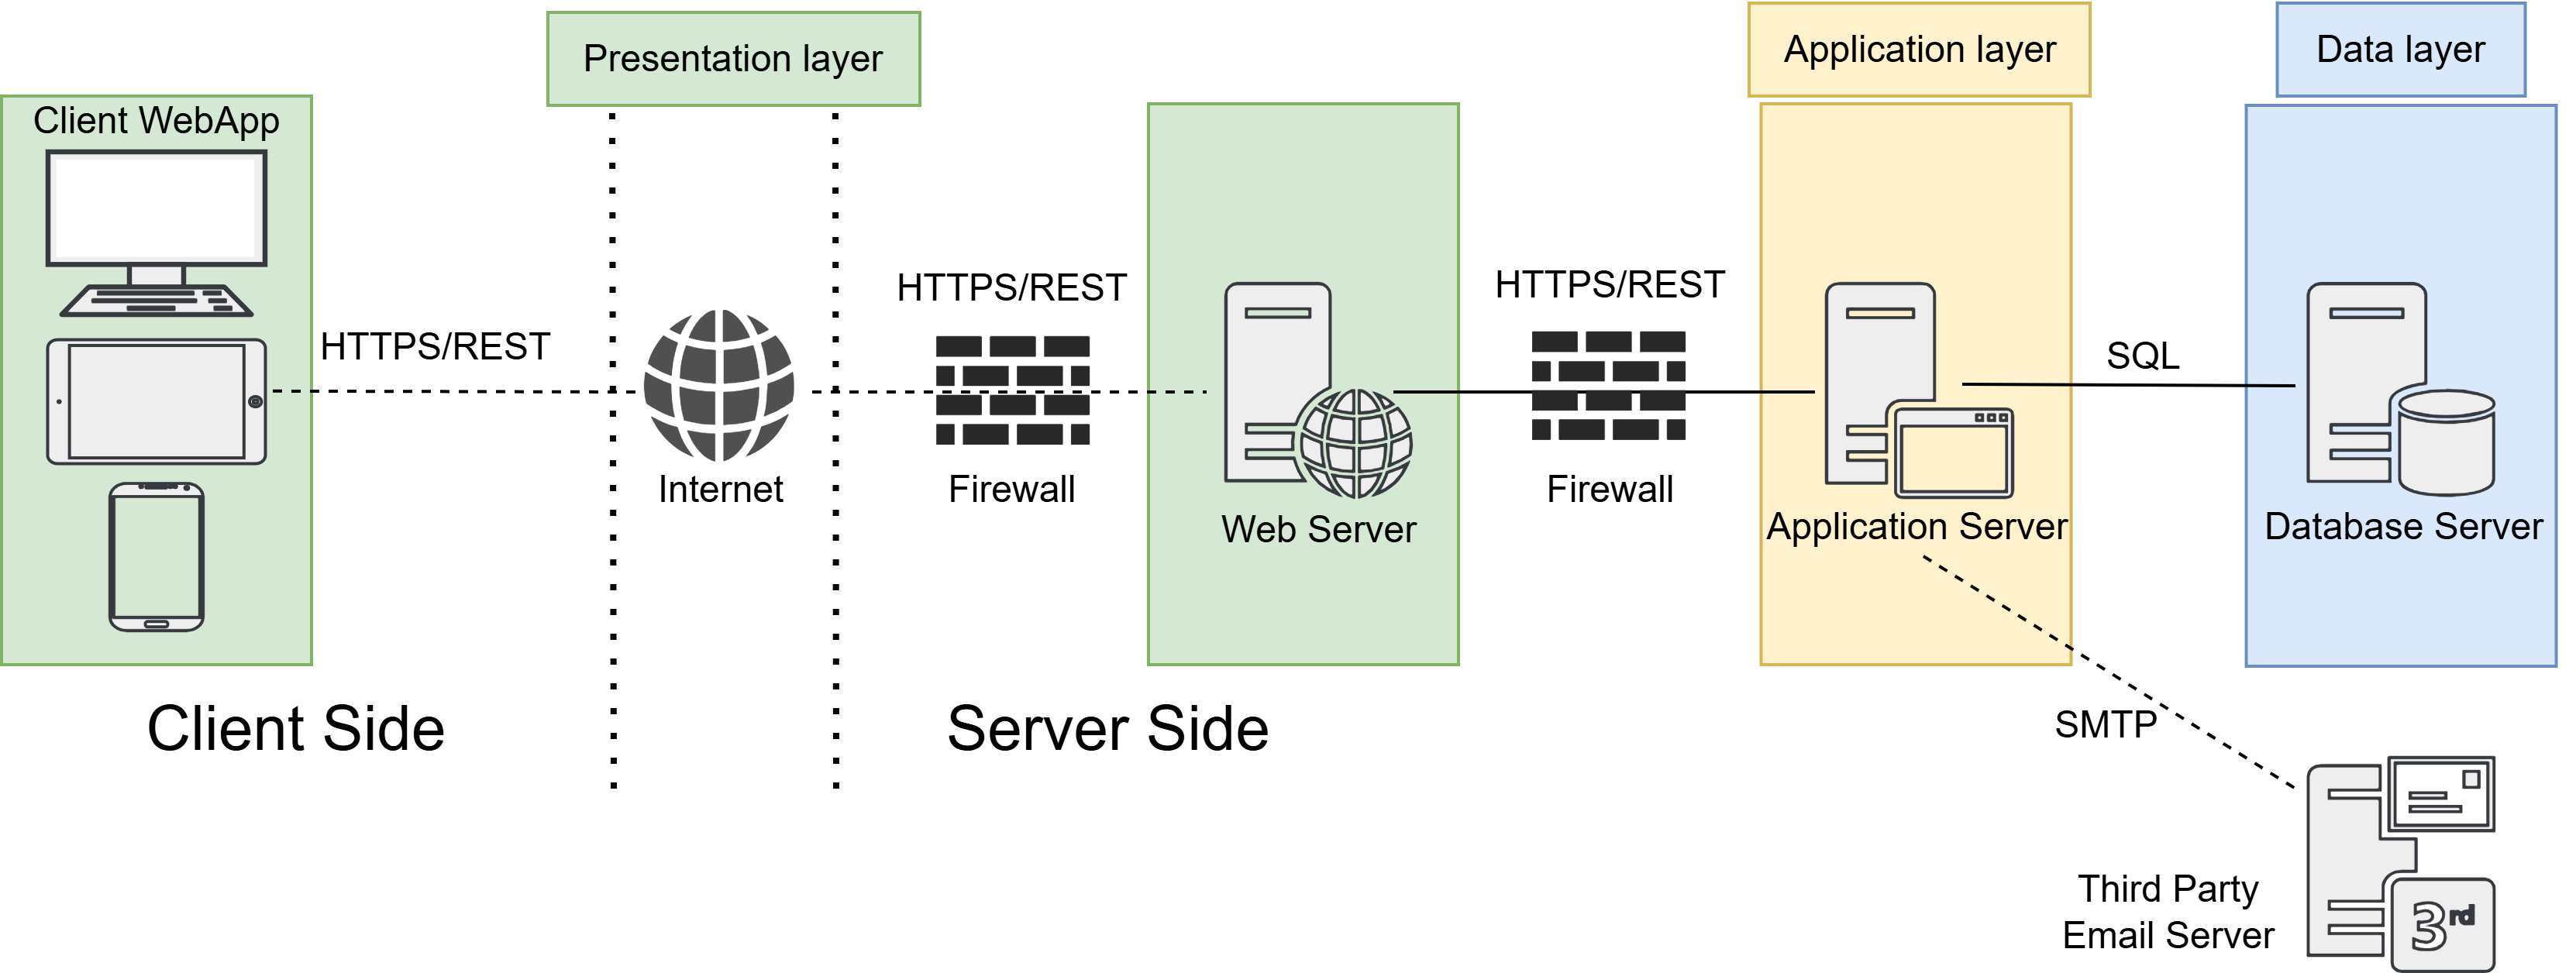
\includegraphics[width=1\textwidth]{Images/tiers_architecture.png}
    \caption{S\&C architectural overview}\label{fig:tiers_architecture}
\end{figure}

In the following paragraph we describe each tier presented in Figure \ref{fig:tiers_architecture}: and what layer it deploys:
\paragraph{Client Side}
\begin{itemize}
    \item \textbf{Web App:} It is the user interface. It will be responsible for managing the user interaction. This means that it will be responsible 
    for hosting part of the presentation layer. 
\end{itemize}

\paragraph{Server Side}
\begin{itemize}
    \item \textbf{Firewall:} It will be responsible for managing the security of the system, by filtering the incoming and outgoing traffic and restricting
    the access based on predefined rules. It will be placed between the Web Server and the Internet and between the Application Server and the Web Server.
    In this way, the web server will reside in a DMZ (Demilitarized Zone), while the application server will resides in a protected internal network.
    \item \textbf{Web Server:} It serves as a gateway between the client and the application server (backend). It will be responsible for hosting part 
    of the presentation layer. For example, it will be responsible for serving the web pages to the client, handling requests routing to the application
    server, managing load balancing, and handling security.
    \item \textbf{Application Server:} It will be responsible for managing the application logic. This means that it will host the application layer. For 
    example, it will be responsible for prcessing the client requests, execute the business logic, and coordinates with the database and email server.
    \item \textbf{Database Server:} It will be responsible for managing the data storage and the data access. This means that it will host the data layer.
    For example, it will be responsible for storing and retrieving the application data, and executing the database queries.
    \item \textbf{Mail Server:} It will be responsible for managing the email communication. This means that it will be responsible for sending emails to 
    the users. It is triggered by the application server.
\end{itemize}

The Figure \ref{fig:tiers_architecture} also shows how the tiers interact with each other. The Web App interacts with the Web Server through HTTPS/REST 
requests; the Web Server interacts with the Application Server through HTTPS/REST calls; the Application Server interacts with the Database Server through 
SQL queries; and the Application Server interacts with the Mail Server through SMTP requests.

\section{Components view}\label{sec:components view}
\subsection{High-level components and interactions}\label{subsec:high-level components and interactions}
\subsection{Low-level components and interactions}\label{subsec:low-level components and interactions}

\section{Deployment view}\label{sec:deployment view}


\section{Component interfaces}\label{sec:component interfaces}


\section{Runtime view}\label{sec:runtime view}


\section{Selected architectural styles and patterns}\label{sec:selected architectural styles and patterns}


\section{Other design decisions}\label{sec:other design decisions}

